\begin{center}
\scalebox{0.56}{
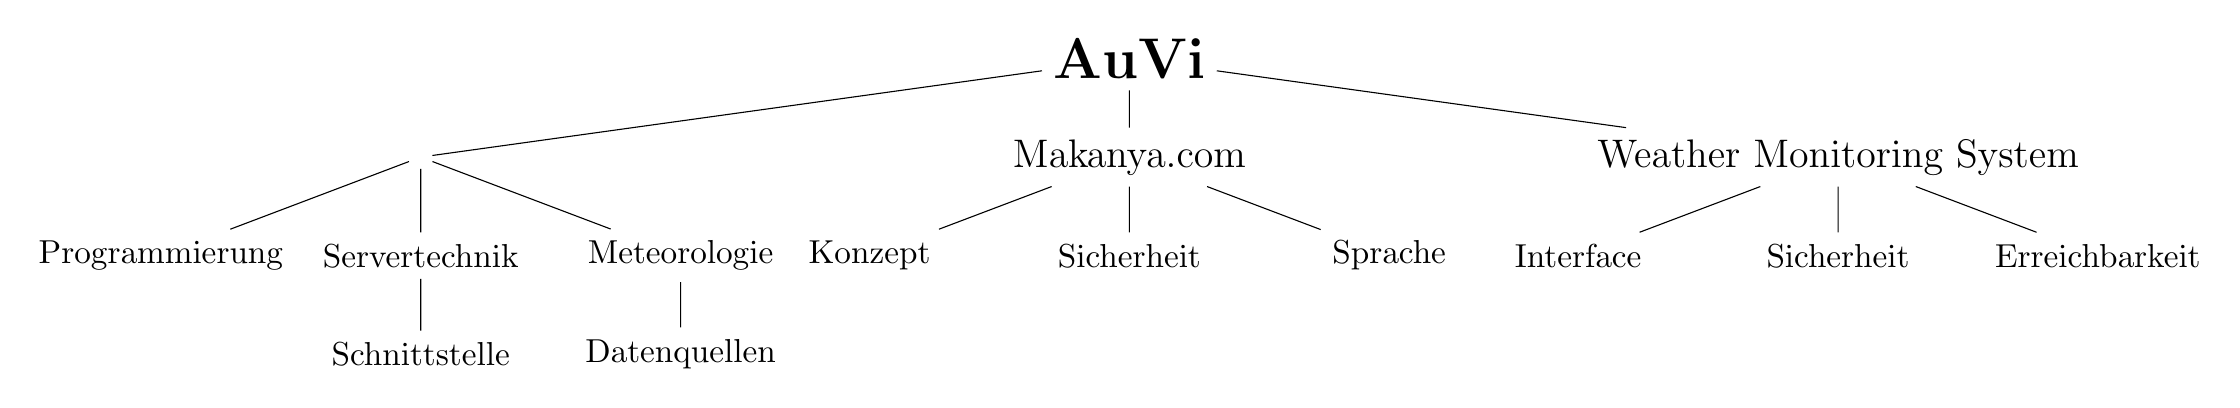
\begin{tikzpicture}[
every node/.style = {scale=1.2},
level 1/.style = {sibling distance = 9cm},
level 2/.style = {sibling distance = 3.3cm},
level 3/.style = {sibling distance = .6cm},
level distance = 1.25cm
]
\node {\LARGE \textbf{AuVi}}
    child { node {\large \vs}
        child { node {Programmierung}}
        child { node {Servertechnik}
            child { node {Schnittstelle}}
        }
        child { node {Meteorologie}
            child { node {Datenquellen}}
        }
    }
    child { node {\large Makanya.com}
        child { node {Konzept}}
        child { node {Sicherheit}}
        child { node {Sprache}}
    }
    child { node {\large Weather Monitoring System}
        child {node {Interface}}
        child {node {Sicherheit}}
        child {node {Erreichbarkeit}}
    };
\end{tikzpicture}
}
\end{center}